\documentclass{article}

\usepackage{stmaryrd}
\usepackage{amssymb}
\usepackage{tikz}
\usetikzlibrary{positioning}

\title{Interaction Diagram - Add Juror to Pool}
\author{ Adam Hammes }

% no page number at bottom
\pagenumbering{gobble}

\begin{document}
\maketitle

\begin{center}

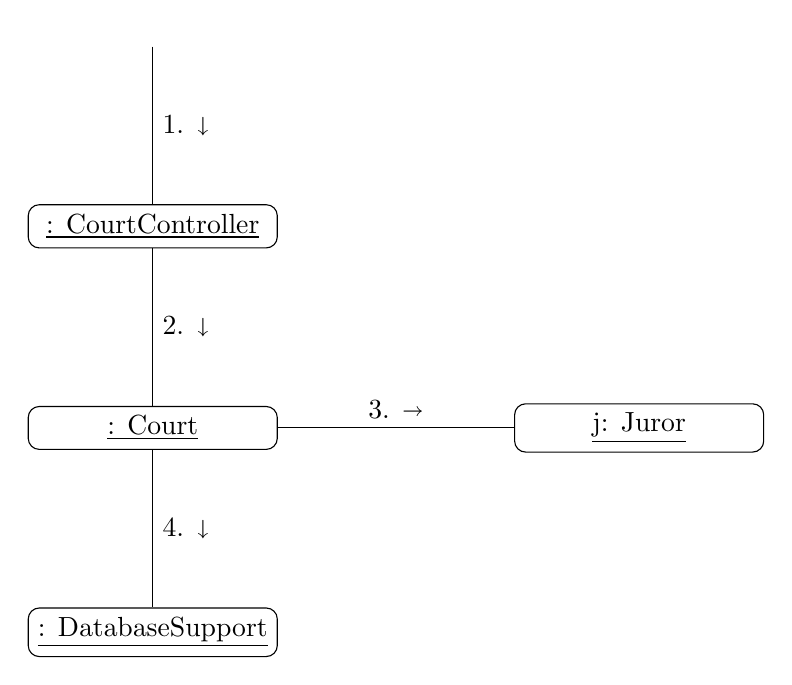
\begin{tikzpicture}[
  auto,
  block/.style = {
    rectangle,
    minimum width = 9em,
    draw=black,
    align=center,
    rounded corners
  }
]
\node[] (start)  {};

\node[block, below = 2cm of start] (controller) {\underline{: CourtController}};
\node[block, below = 2cm of controller] (court) {\underline{: Court}};
\node[block, right = 3cm of court] (juror) {\underline{j: Juror}};
\node[block, below = 2cm of court] (database) {\underline{: DatabaseSupport}};

\draw (start)      -- (controller) node[midway] {1. $\shortdownarrow$};
\draw (controller) -- (court)      node[midway] {2. $\shortdownarrow$};
\draw (court)      -- (juror)      node[midway] {3. $\shortrightarrow$};
\draw (court)      -- (database)   node[midway] {4. $\shortdownarrow$};

\end{tikzpicture}

\vspace{0.5cm}

\begin{enumerate}
  \item \texttt{b:=addJurorToPool(jid:String):boolean}
  \item \texttt{b:=addJurorToPool(jid:String):boolean}
  \item \texttt{create()}
  \item \texttt{b:=putJuror(j):boolean}
\end{enumerate}
\end{center}

\end{document}